\documentclass[12 pt]{article}
\pagestyle{empty}
\addtolength{\topmargin}{-0.9in}
\addtolength{\textheight}{1.9in}
\addtolength{\oddsidemargin}{-0.7in}
\addtolength{\textwidth}{1.4in}
%----------------------------------------------
\usepackage{multicol,
			graphicx,
			amsmath,
			hyperref,
			changepage,
			tikz}
\usepackage{amssymb}
\usepackage{tikz}
\usepackage{enumerate}
%----------------------------------------------			
			


\newcommand{\D}{\displaystyle}
\newcommand{\NN}{\mathbb{N}}
\newcommand{\RR}{\mathbb{R}}
\newcommand{\ZZ}{\mathbb{Z}}

\newcommand{\des}{\text{des}}
\newcommand{\cdes}{\text{cdes}}
\newcommand{\Des}{\text{Des}}

\newcommand{\asc}{\text{asc}}
\newcommand{\Asc}{\text{Asc}}

\newcommand{\Sym}{\mathsf{Sym}}
\newcommand{\Av}{\mathsf{Av}}
\newcommand{\PF}{\mathsf{PF}}

\newcommand{\acts}{\curvearrowright}

%stirling numbers of the second kind
\newcommand{\stirling}{\genfrac{\{}{\}}{0pt}{}}
%Eulerian numbers 
\newcommand{\Eulerian}{\genfrac{\langle}{\rangle}{0pt}{}}

%-------------------------------------------------

\begin{document}
\begin{center}
\textbf{\LARGE Math 596: Homework 7} \\
\end{center}
\begin{center}
	\textbf{\large Due February 28 in class}
\end{center}




\noindent
Complete at least four of the following problems showing all necessary work to support your proof. Please number each problem and carefully write each solution legibly.
\begin{enumerate}
%----------------------------------------------
\item Write down a $2\times 2$ matrix for the linear transformation defined by orthogonal reflection in line that forms an angle of $\theta$ with the positive $x$-axis (depicted below in blue). What matrix do you get when composing this with reflection in the $x$-axis, i.e  $\begin{bmatrix}
	1&0\\0&-1
\end{bmatrix}$?
\[\begin{tikzpicture}[scale=0.75]
	\draw[very thick, blue,latex-latex] (60:-3) to (60:3);
	\draw[latex-latex](3,0) to (-3,0);
	\draw[-latex] (.7,0) arc (0:60:.7) ;
	\node at (30:.4){\footnotesize $\theta$};
\end{tikzpicture}
\]
%-----------------------------------------------
\item  Define $\Sym_n\acts \RR^n$ as in class. Prove that the transpositions are the sole reflections belonging to $\Sym_n$ under the this action.
%----------------------------------------------
\end{enumerate}

\noindent \fbox{\parbox{\textwidth}{
\textbf{Definition} (Group action) Let $G$ be a group with identity  $e$, and let $x$ be a set. We say that $G$ acts on $X$ if, for each $g\in G$ there is a map $g:X\to X$ such that for all $x\in X$
\begin{itemize}
	\item $h(g(x))=(hg)(x)$ for all $h,g\in G$
	\item $e(x)=x$.
\end{itemize}
Equivalently, an action of $G$ on $X$ is a group homomorphism $G\to \Sym(X)$, where $\Sym(X)$ is the set of permutations of $X$.
}}

\begin{enumerate}
\setcounter{enumi}{2}
\item 
\begin{enumerate}[(a)]\item Number the elements of $\Sym_3$ 1 through 6 and let $\Sym_3$ act on itself by left multiplication, what subgroup of $\Sym_6$ the image of this action isomorphic to? 

	\item What about right multiplication of $\Sym_3$ on itself, why does it not satisfy the above definition of a group action? If we instead define for $\sigma, x\in \Sym_3$ an action by right multiplication by the inverse, i.e. $\sigma(x)=x \sigma^{-1}$ show that this does satisfy the above definition.
\end{enumerate}
%----------------------------------------------
\item Let $\Sym_4 $ act on the set of subsets of $[4]$ of size 2
	\[
	\{1,2\}, \{1,3\}, \{1,4\},\{2,3\},\{2,4\},\{3,4\}
	\] by the rule $\sigma\cdot \{i,j\}=\{\sigma(i)\sigma(j)\}$. Can you identify a subgroup of $\Sym_6$ that the image of this action is isomorphic to?
\end{enumerate}
\newpage
\noindent \fbox{\parbox{\textwidth}{
\textbf{Definition} (Dihedral groups) The symmetries of a regular $n$-gon, $n\geq 3$ form a group under composition, called the \textcolor{blue}{\textbf{dihedral group}} of degree $n$ denoted $D_n$.

\[
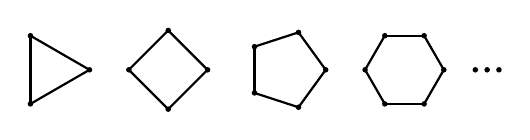
\begin{tikzpicture}[scale=0.5]
\begin{scope}[shift=(0:-10)]
	\foreach \i in {0,1,2}{
		\draw[thick] (120*\i:1) to (120*\i+120:1);
		\fill (120*\i:1) circle (2pt);
	}
\end{scope}
\begin{scope}[shift=(0:-7)]
	\foreach \i in {0,1,2,3}{
		\draw[thick] (90*\i:1) to (90*\i+90:1);
		\fill (90*\i:1) circle (2pt);
	}
\end{scope}

\begin{scope}[shift=(0:-4)]
	\foreach \i in {0,1,2,3,4}{
		\draw[thick] (72*\i:1) to (72*\i+72:1);
		\fill (72*\i:1) circle (2pt);
	}
\end{scope}
\begin{scope}[shift=(0:-1)]
	\foreach \i in {0,1,2,3,4,5}{
		\draw[thick] (60*\i:1) to (60*\i+60:1);
		\fill (60*\i:1) circle (2pt);
	}
\end{scope}
\fill (.8,0) circle (2pt);
\fill (1.1,0) circle (2pt);
\fill (1.4,0) circle (2pt);
\end{tikzpicture}
\]
}}

\begin{enumerate}
\setcounter{enumi}{4}
%----------------------------------------------
\item For an $n$-gon we can label the right-most vertex 1 and continue labeling the vertices in counterclockwise order. For a symmetry we can record it as the permutation on the vertices that it induces. Write out a multiplication table for elements of $D_4$ in this manner.

%----------------------------------------------
\item Every element in $D_n$ can be written as a product of a rotation $r$ counterclockwise rotation by $2\pi/n$ and the reflection in the line connecting vertex 1 to the opposite vertex if $n$ even or midpoint of the opposite  edge if $n$ is odd. Write out a multiplication table for the elements of $D_5$ in this manner.

%----------------------------------------------
\item Find two reflections in the square so that ever element in $D_4$ can be written as a product of these two reflections.

%----------------------------------------------

 
\end{enumerate}

\vfill
%\noindent Selected Hints to Exercises.







\end{document}
